\documentclass{standalone}
\usepackage{tikz}
\usetikzlibrary{patterns, positioning}

\begin{document}
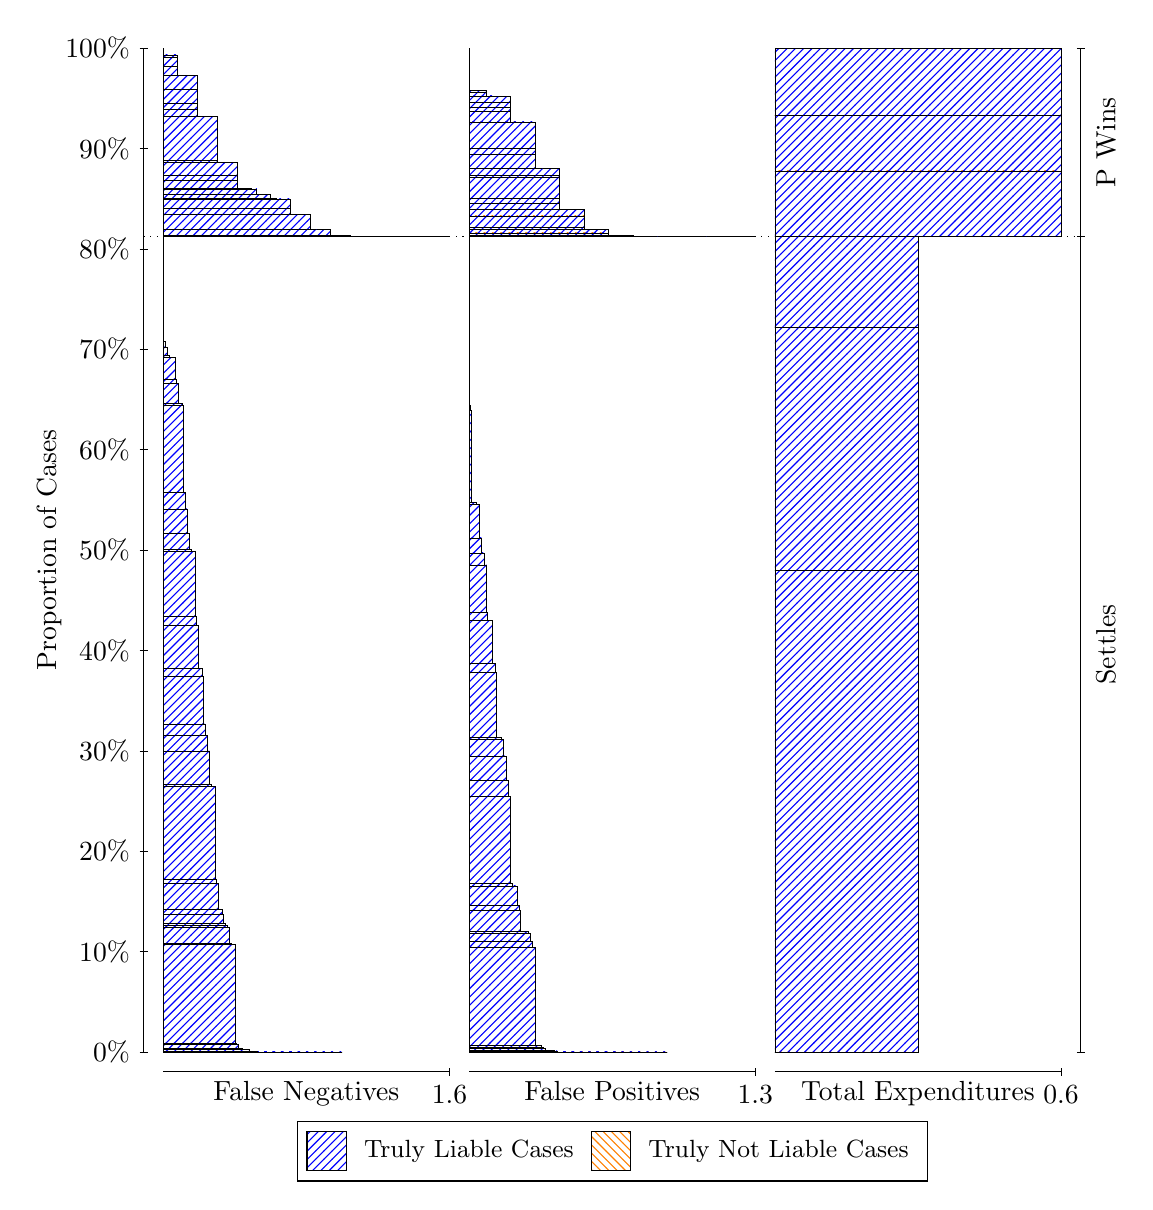
\begin{tikzpicture}
\draw[black, very thin] (1.5,1.75) -- (1.5,14.5);
\node[rotate=90, anchor=center] at (0.3, 8.125) {Proportion of Cases};
\draw[black, very thin] (1.45,1.75) -- (1.55,1.75);
\node[anchor=east] at (1.45, 1.75) {0\%};
\draw[black, very thin] (1.45,3.025) -- (1.55,3.025);
\node[anchor=east] at (1.45, 3.025) {10\%};
\draw[black, very thin] (1.45,4.3) -- (1.55,4.3);
\node[anchor=east] at (1.45, 4.3) {20\%};
\draw[black, very thin] (1.45,5.575) -- (1.55,5.575);
\node[anchor=east] at (1.45, 5.575) {30\%};
\draw[black, very thin] (1.45,6.85) -- (1.55,6.85);
\node[anchor=east] at (1.45, 6.85) {40\%};
\draw[black, very thin] (1.45,8.125) -- (1.55,8.125);
\node[anchor=east] at (1.45, 8.125) {50\%};
\draw[black, very thin] (1.45,9.4) -- (1.55,9.4);
\node[anchor=east] at (1.45, 9.4) {60\%};
\draw[black, very thin] (1.45,10.675) -- (1.55,10.675);
\node[anchor=east] at (1.45, 10.675) {70\%};
\draw[black, very thin] (1.45,11.95) -- (1.55,11.95);
\node[anchor=east] at (1.45, 11.95) {80\%};
\draw[black, very thin] (1.45,13.225) -- (1.55,13.225);
\node[anchor=east] at (1.45, 13.225) {90\%};
\draw[black, very thin] (1.45,14.5) -- (1.55,14.5);
\node[anchor=east] at (1.45, 14.5) {100\%};

\draw[black, very thin] (13.4,1.75) -- (13.4,14.5);
\draw[black, very thin] (13.35,1.75) -- (13.45,1.75);
\node[anchor=west] at (13.35, 1.75) {};
\draw[black, very thin] (13.35,12.104) -- (13.45,12.104);
\node[anchor=west] at (13.35, 12.104) {};
\draw[black, very thin] (13.35,14.5) -- (13.45,14.5);
\node[anchor=west] at (13.35, 14.5) {};

\draw[black, very thin, pattern color=blue, pattern=north east lines] (1.75,1.75) rectangle (4.0208,1.75);
\draw[black, very thin, pattern color=blue, pattern=north east lines] (1.75,1.75) rectangle (3.7937,1.75);
\draw[black, very thin, pattern color=blue, pattern=north east lines] (1.75,1.75) rectangle (3.7685,1.75);
\draw[black, very thin, pattern color=blue, pattern=north east lines] (1.75,1.75) rectangle (3.6802,1.75);
\draw[black, very thin, pattern color=blue, pattern=north east lines] (1.75,1.75) rectangle (3.5667,1.75);
\draw[black, very thin, pattern color=blue, pattern=north east lines] (1.75,1.75) rectangle (3.5414,1.75);
\draw[black, very thin, pattern color=blue, pattern=north east lines] (1.75,1.75) rectangle (3.5162,1.75);
\draw[black, very thin, pattern color=blue, pattern=north east lines] (1.75,1.75) rectangle (3.4531,1.75);
\draw[black, very thin, pattern color=blue, pattern=north east lines] (1.75,1.75) rectangle (3.4279,1.75);
\draw[black, very thin, pattern color=blue, pattern=north east lines] (1.75,1.75) rectangle (3.3396,1.75);
\draw[black, very thin, pattern color=blue, pattern=north east lines] (1.75,1.75) rectangle (3.3144,1.75);
\draw[black, very thin, pattern color=blue, pattern=north east lines] (1.75,1.75) rectangle (3.2891,1.75);
\draw[black, very thin, pattern color=blue, pattern=north east lines] (1.75,1.75) rectangle (3.2639,1.75);
\draw[black, very thin, pattern color=blue, pattern=north east lines] (1.75,1.75) rectangle (3.2008,1.75);
\draw[black, very thin, pattern color=blue, pattern=north east lines] (1.75,1.75) rectangle (3.1756,1.75);
\draw[black, very thin, pattern color=blue, pattern=north east lines] (1.75,1.75) rectangle (3.1125,1.75);
\draw[black, very thin, pattern color=blue, pattern=north east lines] (1.75,1.75) rectangle (3.0873,1.7506);
\draw[black, very thin, pattern color=blue, pattern=north east lines] (1.75,1.7506) rectangle (3.062,1.7506);
\draw[black, very thin, pattern color=blue, pattern=north east lines] (1.75,1.7506) rectangle (3.0368,1.7506);
\draw[black, very thin, pattern color=blue, pattern=north east lines] (1.75,1.7506) rectangle (3.0116,1.7507);
\draw[black, very thin, pattern color=blue, pattern=north east lines] (1.75,1.7507) rectangle (2.999,1.7511);
\draw[black, very thin, pattern color=blue, pattern=north east lines] (1.75,1.7511) rectangle (2.9485,1.7536);
\draw[black, very thin, pattern color=blue, pattern=north east lines] (1.75,1.7536) rectangle (2.9233,1.7538);
\draw[black, very thin, pattern color=blue, pattern=north east lines] (1.75,1.7538) rectangle (2.8602,1.7541);
\draw[black, very thin, pattern color=blue, pattern=north east lines] (1.75,1.7541) rectangle (2.835,1.7782);
\draw[black, very thin, pattern color=blue, pattern=north east lines] (1.75,1.7782) rectangle (2.8097,1.7787);
\draw[black, very thin, pattern color=blue, pattern=north east lines] (1.75,1.7787) rectangle (2.7845,1.7792);
\draw[black, very thin, pattern color=blue, pattern=north east lines] (1.75,1.7792) rectangle (2.7593,1.7849);
\draw[black, very thin, pattern color=blue, pattern=north east lines] (1.75,1.7849) rectangle (2.7466,1.7924);
\draw[black, very thin, pattern color=blue, pattern=north east lines] (1.75,1.7924) rectangle (2.6962,1.8506);
\draw[black, very thin, pattern color=blue, pattern=north east lines] (1.75,1.8506) rectangle (2.6709,1.8575);
\draw[black, very thin, pattern color=blue, pattern=north east lines] (1.75,1.8575) rectangle (2.6583,3.1206);
\draw[black, very thin, pattern color=blue, pattern=north east lines] (1.75,3.1206) rectangle (2.6079,3.1261);
\draw[black, very thin, pattern color=blue, pattern=north east lines] (1.75,3.1261) rectangle (2.5826,3.3375);
\draw[black, very thin, pattern color=blue, pattern=north east lines] (1.75,3.3375) rectangle (2.5574,3.3609);
\draw[black, very thin, pattern color=blue, pattern=north east lines] (1.75,3.3609) rectangle (2.5322,3.3815);
\draw[black, very thin, pattern color=blue, pattern=north east lines] (1.75,3.3815) rectangle (2.5069,3.5027);
\draw[black, very thin, pattern color=blue, pattern=north east lines] (1.75,3.5027) rectangle (2.4943,3.5563);
\draw[black, very thin, pattern color=blue, pattern=north east lines] (1.75,3.5563) rectangle (2.4439,3.8903);
\draw[black, very thin, pattern color=blue, pattern=north east lines] (1.75,3.8903) rectangle (2.4186,3.9486);
\draw[black, very thin, pattern color=blue, pattern=north east lines] (1.75,3.9486) rectangle (2.406,5.1245);
\draw[black, very thin, pattern color=blue, pattern=north east lines] (1.75,5.1245) rectangle (2.3556,5.1507);
\draw[black, very thin, pattern color=blue, pattern=north east lines] (1.75,5.1507) rectangle (2.3303,5.5742);
\draw[black, very thin, pattern color=blue, pattern=north east lines] (1.75,5.5742) rectangle (2.3051,5.7667);
\draw[black, very thin, pattern color=blue, pattern=north east lines] (1.75,5.7667) rectangle (2.2799,5.9173);
\draw[black, very thin, pattern color=blue, pattern=north east lines] (1.75,5.9173) rectangle (2.2546,6.5235);
\draw[black, very thin, pattern color=blue, pattern=north east lines] (1.75,6.5235) rectangle (2.242,6.6186);
\draw[black, very thin, pattern color=blue, pattern=north east lines] (1.75,6.6186) rectangle (2.1916,7.1644);
\draw[black, very thin, pattern color=blue, pattern=north east lines] (1.75,7.1644) rectangle (2.1663,7.2856);
\draw[black, very thin, pattern color=blue, pattern=north east lines] (1.75,7.2856) rectangle (2.1537,8.1057);
\draw[black, very thin, pattern color=blue, pattern=north east lines] (1.75,8.1057) rectangle (2.1032,8.1314);
\draw[black, very thin, pattern color=blue, pattern=north east lines] (1.75,8.1314) rectangle (2.078,8.3432);
\draw[black, very thin, pattern color=blue, pattern=north east lines] (1.75,8.3432) rectangle (2.0528,8.6483);
\draw[black, very thin, pattern color=blue, pattern=north east lines] (1.75,8.6483) rectangle (2.0275,8.8621);
\draw[black, very thin, pattern color=blue, pattern=north east lines] (1.75,8.8621) rectangle (2.0023,9.9611);
\draw[black, very thin, pattern color=blue, pattern=north east lines] (1.75,9.9611) rectangle (1.9897,9.9937);
\draw[black, very thin, pattern color=blue, pattern=north east lines] (1.75,9.9937) rectangle (1.9392,10.239);
\draw[black, very thin, pattern color=blue, pattern=north east lines] (1.75,10.239) rectangle (1.914,10.298);
\draw[black, very thin, pattern color=blue, pattern=north east lines] (1.75,10.298) rectangle (1.9014,10.57);
\draw[black, very thin, pattern color=blue, pattern=north east lines] (1.75,10.57) rectangle (1.8509,10.575);
\draw[black, very thin, pattern color=blue, pattern=north east lines] (1.75,10.575) rectangle (1.8257,10.599);
\draw[black, very thin, pattern color=blue, pattern=north east lines] (1.75,10.599) rectangle (1.8005,10.694);
\draw[black, very thin, pattern color=blue, pattern=north east lines] (1.75,10.694) rectangle (1.7752,10.77);
\draw[black, very thin, pattern color=orange, pattern=north west lines] (1.75,10.77) rectangle (1.75,10.77);
\draw[black, very thin, pattern color=blue, pattern=north east lines] (1.75,10.77) rectangle (1.75,12.104);
\draw[black, very thin, pattern color=blue, pattern=north east lines] (1.75,12.104) rectangle (5.3833,12.104);
\draw[black, very thin, pattern color=blue, pattern=north east lines] (1.75,12.104) rectangle (5.131,12.104);
\draw[black, very thin, pattern color=blue, pattern=north east lines] (1.75,12.104) rectangle (4.8787,12.104);
\draw[black, very thin, pattern color=blue, pattern=north east lines] (1.75,12.104) rectangle (4.6264,12.104);
\draw[black, very thin, pattern color=blue, pattern=north east lines] (1.75,12.104) rectangle (4.3741,12.106);
\draw[black, very thin, pattern color=blue, pattern=north east lines] (1.75,12.106) rectangle (4.1975,12.106);
\draw[black, very thin, pattern color=blue, pattern=north east lines] (1.75,12.106) rectangle (4.1218,12.113);
\draw[black, very thin, pattern color=blue, pattern=north east lines] (1.75,12.113) rectangle (4.1218,12.121);
\draw[black, very thin, pattern color=blue, pattern=north east lines] (1.75,12.121) rectangle (3.9451,12.121);
\draw[black, very thin, pattern color=blue, pattern=north east lines] (1.75,12.121) rectangle (3.9451,12.121);
\draw[black, very thin, pattern color=blue, pattern=north east lines] (1.75,12.121) rectangle (3.8694,12.195);
\draw[black, very thin, pattern color=blue, pattern=north east lines] (1.75,12.195) rectangle (3.6928,12.195);
\draw[black, very thin, pattern color=blue, pattern=north east lines] (1.75,12.195) rectangle (3.6928,12.195);
\draw[black, very thin, pattern color=blue, pattern=north east lines] (1.75,12.195) rectangle (3.6171,12.389);
\draw[black, very thin, pattern color=blue, pattern=north east lines] (1.75,12.389) rectangle (3.4405,12.39);
\draw[black, very thin, pattern color=blue, pattern=north east lines] (1.75,12.39) rectangle (3.3648,12.462);
\draw[black, very thin, pattern color=blue, pattern=north east lines] (1.75,12.462) rectangle (3.3648,12.583);
\draw[black, very thin, pattern color=blue, pattern=north east lines] (1.75,12.583) rectangle (3.1882,12.589);
\draw[black, very thin, pattern color=blue, pattern=north east lines] (1.75,12.589) rectangle (3.1125,12.645);
\draw[black, very thin, pattern color=blue, pattern=north east lines] (1.75,12.645) rectangle (2.9359,12.645);
\draw[black, very thin, pattern color=blue, pattern=north east lines] (1.75,12.645) rectangle (2.9359,12.712);
\draw[black, very thin, pattern color=blue, pattern=north east lines] (1.75,12.712) rectangle (2.8602,12.717);
\draw[black, very thin, pattern color=blue, pattern=north east lines] (1.75,12.717) rectangle (2.6836,12.721);
\draw[black, very thin, pattern color=blue, pattern=north east lines] (1.75,12.721) rectangle (2.6836,12.815);
\draw[black, very thin, pattern color=blue, pattern=north east lines] (1.75,12.815) rectangle (2.6836,12.89);
\draw[black, very thin, pattern color=blue, pattern=north east lines] (1.75,12.89) rectangle (2.6836,13.043);
\draw[black, very thin, pattern color=blue, pattern=north east lines] (1.75,13.043) rectangle (2.6079,13.043);
\draw[black, very thin, pattern color=blue, pattern=north east lines] (1.75,13.043) rectangle (2.4312,13.076);
\draw[black, very thin, pattern color=blue, pattern=north east lines] (1.75,13.076) rectangle (2.4312,13.636);
\draw[black, very thin, pattern color=blue, pattern=north east lines] (1.75,13.636) rectangle (2.3556,13.636);
\draw[black, very thin, pattern color=blue, pattern=north east lines] (1.75,13.636) rectangle (2.1789,13.717);
\draw[black, very thin, pattern color=blue, pattern=north east lines] (1.75,13.717) rectangle (2.1789,13.802);
\draw[black, very thin, pattern color=blue, pattern=north east lines] (1.75,13.802) rectangle (2.1789,13.972);
\draw[black, very thin, pattern color=blue, pattern=north east lines] (1.75,13.972) rectangle (2.1789,14.151);
\draw[black, very thin, pattern color=blue, pattern=north east lines] (1.75,14.151) rectangle (2.1032,14.151);
\draw[black, very thin, pattern color=blue, pattern=north east lines] (1.75,14.151) rectangle (1.9266,14.262);
\draw[black, very thin, pattern color=blue, pattern=north east lines] (1.75,14.262) rectangle (1.9266,14.378);
\draw[black, very thin, pattern color=blue, pattern=north east lines] (1.75,14.378) rectangle (1.9266,14.412);
\draw[black, very thin, pattern color=orange, pattern=north west lines] (1.75,14.412) rectangle (1.75,14.412);
\draw[black, very thin, pattern color=blue, pattern=north east lines] (1.75,14.412) rectangle (1.75,14.5);
\draw[black, very thin, pattern color=orange, pattern=north west lines] (5.6333,1.75) rectangle (8.1487,1.75);
\draw[black, very thin, pattern color=blue, pattern=north east lines] (5.6333,1.75) rectangle (8.1487,1.75);
\draw[black, very thin, pattern color=blue, pattern=north east lines] (5.6333,1.75) rectangle (7.8382,1.75);
\draw[black, very thin, pattern color=orange, pattern=north west lines] (5.6333,1.75) rectangle (7.7295,1.75);
\draw[black, very thin, pattern color=blue, pattern=north east lines] (5.6333,1.75) rectangle (7.7295,1.75);
\draw[black, very thin, pattern color=orange, pattern=north west lines] (5.6333,1.75) rectangle (7.5897,1.75);
\draw[black, very thin, pattern color=blue, pattern=north east lines] (5.6333,1.75) rectangle (7.5897,1.75);
\draw[black, very thin, pattern color=blue, pattern=north east lines] (5.6333,1.75) rectangle (7.5276,1.75);
\draw[black, very thin, pattern color=blue, pattern=north east lines] (5.6333,1.75) rectangle (7.4189,1.75);
\draw[black, very thin, pattern color=orange, pattern=north west lines] (5.6333,1.75) rectangle (7.3103,1.75);
\draw[black, very thin, pattern color=blue, pattern=north east lines] (5.6333,1.75) rectangle (7.3103,1.75);
\draw[black, very thin, pattern color=blue, pattern=north east lines] (5.6333,1.75) rectangle (7.2792,1.75);
\draw[black, very thin, pattern color=blue, pattern=north east lines] (5.6333,1.75) rectangle (7.2171,1.75);
\draw[black, very thin, pattern color=orange, pattern=north west lines] (5.6333,1.75) rectangle (7.1705,1.75);
\draw[black, very thin, pattern color=blue, pattern=north east lines] (5.6333,1.75) rectangle (7.1705,1.75);
\draw[black, very thin, pattern color=blue, pattern=north east lines] (5.6333,1.75) rectangle (7.1084,1.75);
\draw[black, very thin, pattern color=orange, pattern=north west lines] (5.6333,1.75) rectangle (7.0308,1.75);
\draw[black, very thin, pattern color=blue, pattern=north east lines] (5.6333,1.75) rectangle (7.0308,1.7501);
\draw[black, very thin, pattern color=blue, pattern=north east lines] (5.6333,1.7501) rectangle (6.9997,1.7501);
\draw[black, very thin, pattern color=blue, pattern=north east lines] (5.6333,1.7501) rectangle (6.9687,1.7501);
\draw[black, very thin, pattern color=blue, pattern=north east lines] (5.6333,1.7501) rectangle (6.9066,1.7506);
\draw[black, very thin, pattern color=orange, pattern=north west lines] (5.6333,1.7506) rectangle (6.891,1.7506);
\draw[black, very thin, pattern color=blue, pattern=north east lines] (5.6333,1.7506) rectangle (6.891,1.7511);
\draw[black, very thin, pattern color=blue, pattern=north east lines] (5.6333,1.7511) rectangle (6.86,1.7517);
\draw[black, very thin, pattern color=blue, pattern=north east lines] (5.6333,1.7517) rectangle (6.7979,1.7517);
\draw[black, very thin, pattern color=orange, pattern=north west lines] (5.6333,1.7517) rectangle (6.7513,1.7517);
\draw[black, very thin, pattern color=blue, pattern=north east lines] (5.6333,1.7517) rectangle (6.7513,1.7626);
\draw[black, very thin, pattern color=blue, pattern=north east lines] (5.6333,1.7626) rectangle (6.7202,1.7685);
\draw[black, very thin, pattern color=blue, pattern=north east lines] (5.6333,1.7685) rectangle (6.6892,1.769);
\draw[black, very thin, pattern color=blue, pattern=north east lines] (5.6333,1.769) rectangle (6.6581,1.7692);
\draw[black, very thin, pattern color=blue, pattern=north east lines] (5.6333,1.7692) rectangle (6.596,1.7955);
\draw[black, very thin, pattern color=blue, pattern=north east lines] (5.6333,1.7955) rectangle (6.5805,1.8034);
\draw[black, very thin, pattern color=blue, pattern=north east lines] (5.6333,1.8034) rectangle (6.5494,1.8294);
\draw[black, very thin, pattern color=blue, pattern=north east lines] (5.6333,1.8294) rectangle (6.4873,1.8314);
\draw[black, very thin, pattern color=orange, pattern=north west lines] (5.6333,1.8314) rectangle (6.4718,1.8314);
\draw[black, very thin, pattern color=blue, pattern=north east lines] (5.6333,1.8314) rectangle (6.4718,3.0836);
\draw[black, very thin, pattern color=blue, pattern=north east lines] (5.6333,3.0836) rectangle (6.4407,3.1604);
\draw[black, very thin, pattern color=blue, pattern=north east lines] (5.6333,3.1604) rectangle (6.4097,3.2548);
\draw[black, very thin, pattern color=blue, pattern=north east lines] (5.6333,3.2548) rectangle (6.3786,3.2787);
\draw[black, very thin, pattern color=blue, pattern=north east lines] (5.6333,3.2787) rectangle (6.3476,3.2836);
\draw[black, very thin, pattern color=blue, pattern=north east lines] (5.6333,3.2836) rectangle (6.2855,3.5555);
\draw[black, very thin, pattern color=blue, pattern=north east lines] (5.6333,3.5555) rectangle (6.2699,3.6146);
\draw[black, very thin, pattern color=blue, pattern=north east lines] (5.6333,3.6146) rectangle (6.2389,3.8602);
\draw[black, very thin, pattern color=blue, pattern=north east lines] (5.6333,3.8602) rectangle (6.1768,3.8929);
\draw[black, very thin, pattern color=blue, pattern=north east lines] (5.6333,3.8929) rectangle (6.1613,4.9918);
\draw[black, very thin, pattern color=blue, pattern=north east lines] (5.6333,4.9918) rectangle (6.1302,5.2057);
\draw[black, very thin, pattern color=blue, pattern=north east lines] (5.6333,5.2057) rectangle (6.0991,5.5108);
\draw[black, very thin, pattern color=blue, pattern=north east lines] (5.6333,5.5108) rectangle (6.0681,5.7225);
\draw[black, very thin, pattern color=blue, pattern=north east lines] (5.6333,5.7225) rectangle (6.037,5.7483);
\draw[black, very thin, pattern color=blue, pattern=north east lines] (5.6333,5.7483) rectangle (5.9749,6.5683);
\draw[black, very thin, pattern color=blue, pattern=north east lines] (5.6333,6.5683) rectangle (5.9594,6.6896);
\draw[black, very thin, pattern color=blue, pattern=north east lines] (5.6333,6.6896) rectangle (5.9283,7.2354);
\draw[black, very thin, pattern color=blue, pattern=north east lines] (5.6333,7.2354) rectangle (5.8662,7.3304);
\draw[black, very thin, pattern color=blue, pattern=north east lines] (5.6333,7.3304) rectangle (5.8507,7.9366);
\draw[black, very thin, pattern color=blue, pattern=north east lines] (5.6333,7.9366) rectangle (5.8197,8.0872);
\draw[black, very thin, pattern color=blue, pattern=north east lines] (5.6333,8.0872) rectangle (5.7886,8.2797);
\draw[black, very thin, pattern color=blue, pattern=north east lines] (5.6333,8.2797) rectangle (5.7575,8.7033);
\draw[black, very thin, pattern color=blue, pattern=north east lines] (5.6333,8.7033) rectangle (5.7265,8.7295);
\draw[black, very thin, pattern color=blue, pattern=north east lines] (5.6333,8.7295) rectangle (5.6644,9.9053);
\draw[black, very thin, pattern color=blue, pattern=north east lines] (5.6333,9.9053) rectangle (5.6489,9.9637);
\draw[black, very thin, pattern color=blue, pattern=north east lines] (5.6333,9.9637) rectangle (5.6333,12.104);
\draw[black, very thin, pattern color=orange, pattern=north west lines] (5.6333,12.104) rectangle (9.2667,12.104);
\draw[black, very thin, pattern color=blue, pattern=north east lines] (5.6333,12.104) rectangle (9.2667,12.104);
\draw[black, very thin, pattern color=orange, pattern=north west lines] (5.6333,12.104) rectangle (8.9561,12.104);
\draw[black, very thin, pattern color=blue, pattern=north east lines] (5.6333,12.104) rectangle (8.9561,12.104);
\draw[black, very thin, pattern color=blue, pattern=north east lines] (5.6333,12.104) rectangle (8.6456,12.104);
\draw[black, very thin, pattern color=orange, pattern=north west lines] (5.6333,12.104) rectangle (8.6456,12.104);
\draw[black, very thin, pattern color=blue, pattern=north east lines] (5.6333,12.104) rectangle (8.6456,12.104);
\draw[black, very thin, pattern color=blue, pattern=north east lines] (5.6333,12.104) rectangle (8.335,12.104);
\draw[black, very thin, pattern color=blue, pattern=north east lines] (5.6333,12.104) rectangle (8.335,12.104);
\draw[black, very thin, pattern color=orange, pattern=north west lines] (5.6333,12.104) rectangle (8.335,12.104);
\draw[black, very thin, pattern color=blue, pattern=north east lines] (5.6333,12.104) rectangle (8.335,12.104);
\draw[black, very thin, pattern color=orange, pattern=north west lines] (5.6333,12.104) rectangle (8.0245,12.104);
\draw[black, very thin, pattern color=blue, pattern=north east lines] (5.6333,12.104) rectangle (8.0245,12.105);
\draw[black, very thin, pattern color=blue, pattern=north east lines] (5.6333,12.105) rectangle (8.0245,12.105);
\draw[black, very thin, pattern color=blue, pattern=north east lines] (5.6333,12.105) rectangle (8.0245,12.105);
\draw[black, very thin, pattern color=orange, pattern=north west lines] (5.6333,12.105) rectangle (7.714,12.105);
\draw[black, very thin, pattern color=blue, pattern=north east lines] (5.6333,12.105) rectangle (7.714,12.114);
\draw[black, very thin, pattern color=blue, pattern=north east lines] (5.6333,12.114) rectangle (7.714,12.117);
\draw[black, very thin, pattern color=blue, pattern=north east lines] (5.6333,12.117) rectangle (7.4034,12.151);
\draw[black, very thin, pattern color=orange, pattern=north west lines] (5.6333,12.151) rectangle (7.4034,12.151);
\draw[black, very thin, pattern color=blue, pattern=north east lines] (5.6333,12.151) rectangle (7.4034,12.192);
\draw[black, very thin, pattern color=blue, pattern=north east lines] (5.6333,12.192) rectangle (7.0929,12.226);
\draw[black, very thin, pattern color=blue, pattern=north east lines] (5.6333,12.226) rectangle (7.0929,12.369);
\draw[black, very thin, pattern color=orange, pattern=north west lines] (5.6333,12.369) rectangle (7.0929,12.369);
\draw[black, very thin, pattern color=blue, pattern=north east lines] (5.6333,12.369) rectangle (7.0929,12.453);
\draw[black, very thin, pattern color=orange, pattern=north west lines] (5.6333,12.453) rectangle (6.8755,12.453);
\draw[black, very thin, pattern color=blue, pattern=north east lines] (5.6333,12.453) rectangle (6.8755,12.453);
\draw[black, very thin, pattern color=blue, pattern=north east lines] (5.6333,12.453) rectangle (6.7823,12.525);
\draw[black, very thin, pattern color=blue, pattern=north east lines] (5.6333,12.525) rectangle (6.7823,12.59);
\draw[black, very thin, pattern color=blue, pattern=north east lines] (5.6333,12.59) rectangle (6.7823,12.862);
\draw[black, very thin, pattern color=blue, pattern=north east lines] (5.6333,12.862) rectangle (6.7823,12.883);
\draw[black, very thin, pattern color=blue, pattern=north east lines] (5.6333,12.883) rectangle (6.7823,12.968);
\draw[black, very thin, pattern color=orange, pattern=north west lines] (5.6333,12.968) rectangle (6.565,12.968);
\draw[black, very thin, pattern color=blue, pattern=north east lines] (5.6333,12.968) rectangle (6.565,12.968);
\draw[black, very thin, pattern color=blue, pattern=north east lines] (5.6333,12.968) rectangle (6.4718,13.152);
\draw[black, very thin, pattern color=blue, pattern=north east lines] (5.6333,13.152) rectangle (6.4718,13.224);
\draw[black, very thin, pattern color=blue, pattern=north east lines] (5.6333,13.224) rectangle (6.4718,13.561);
\draw[black, very thin, pattern color=orange, pattern=north west lines] (5.6333,13.561) rectangle (6.2544,13.561);
\draw[black, very thin, pattern color=blue, pattern=north east lines] (5.6333,13.561) rectangle (6.2544,13.561);
\draw[black, very thin, pattern color=blue, pattern=north east lines] (5.6333,13.561) rectangle (6.1613,13.691);
\draw[black, very thin, pattern color=blue, pattern=north east lines] (5.6333,13.691) rectangle (6.1613,13.747);
\draw[black, very thin, pattern color=blue, pattern=north east lines] (5.6333,13.747) rectangle (6.1613,13.805);
\draw[black, very thin, pattern color=blue, pattern=north east lines] (5.6333,13.805) rectangle (6.1613,13.887);
\draw[black, very thin, pattern color=orange, pattern=north west lines] (5.6333,13.887) rectangle (5.9439,13.887);
\draw[black, very thin, pattern color=blue, pattern=north east lines] (5.6333,13.887) rectangle (5.9439,13.892);
\draw[black, very thin, pattern color=blue, pattern=north east lines] (5.6333,13.892) rectangle (5.8507,13.936);
\draw[black, very thin, pattern color=blue, pattern=north east lines] (5.6333,13.936) rectangle (5.8507,13.959);
\draw[black, very thin, pattern color=orange, pattern=north west lines] (5.6333,13.959) rectangle (5.6333,13.959);
\draw[black, very thin, pattern color=blue, pattern=north east lines] (5.6333,13.959) rectangle (5.6333,14.5);
\draw[black, very thin, pattern color=orange, pattern=north west lines] (9.5167,1.75) rectangle (11.333,1.75);
\draw[black, very thin, pattern color=blue, pattern=north east lines] (9.5167,1.75) rectangle (11.333,7.8697);
\draw[black, very thin, pattern color=orange, pattern=north west lines] (9.5167,7.8697) rectangle (11.333,7.8697);
\draw[black, very thin, pattern color=blue, pattern=north east lines] (9.5167,7.8697) rectangle (11.333,10.954);
\draw[black, very thin, pattern color=orange, pattern=north west lines] (9.5167,10.954) rectangle (11.333,10.954);
\draw[black, very thin, pattern color=blue, pattern=north east lines] (9.5167,10.954) rectangle (11.333,12.104);
\draw[black, very thin, pattern color=orange, pattern=north west lines] (9.5167,12.104) rectangle (13.15,12.104);
\draw[black, very thin, pattern color=blue, pattern=north east lines] (9.5167,12.104) rectangle (13.15,12.94);
\draw[black, very thin, pattern color=orange, pattern=north west lines] (9.5167,12.94) rectangle (13.15,12.94);
\draw[black, very thin, pattern color=blue, pattern=north east lines] (9.5167,12.94) rectangle (13.15,13.641);
\draw[black, very thin, pattern color=orange, pattern=north west lines] (9.5167,13.641) rectangle (13.15,13.641);
\draw[black, very thin, pattern color=blue, pattern=north east lines] (9.5167,13.641) rectangle (13.15,14.5);
\draw[black, dotted] (1.5,12.104) -- (13.4,12.104);
\draw[black, very thin] (1.75,1.5) -- (5.3833,1.5);
\node[anchor=north] at (3.5667, 1.5) {False Negatives};
\draw[black, very thin] (5.3833,1.45) -- (5.3833,1.55);
\node[anchor=north] at (5.3833, 1.45) {1.6};

\draw[black, very thin] (5.6333,1.5) -- (9.2667,1.5);
\node[anchor=north] at (7.45, 1.5) {False Positives};
\draw[black, very thin] (9.2667,1.45) -- (9.2667,1.55);
\node[anchor=north] at (9.2667, 1.45) {1.3};

\draw[black, very thin] (9.5167,1.5) -- (13.15,1.5);
\node[anchor=north] at (11.333, 1.5) {Total Expenditures};
\draw[black, very thin] (13.15,1.45) -- (13.15,1.55);
\node[anchor=north] at (13.15, 1.45) {0.6};

\node[black, centered, rotate=90] at (13.72, 6.927) {Settles};
\node[black, centered, rotate=90] at (13.72, 13.302) {P Wins};

\draw (7.449999999999999,1.5) node[draw=none] (baseCoordinate) {};
\begin{scope}[align=center]
        \matrix[scale=0.5, draw=black, below=0.5cm of baseCoordinate, nodes={draw}, column sep=0.1cm]{
            \node[rectangle, draw, minimum width=0.5cm, minimum height=0.5cm, pattern=north east lines, pattern color=blue] {}; &
            \node[draw=none, font=\small] (B) {Truly Liable Cases}; &
            \node[rectangle, draw, minimum width=0.5cm, minimum height=0.5cm, pattern=north west lines, pattern color=orange] {}; &
            \node[draw=none, font=\small] (B) {Truly Not Liable Cases}; \\
            };
\end{scope}

\end{tikzpicture}
\end{document}